

\tikzset{every picture/.style={line width=0.75pt}} %set default line width to 0.75pt        

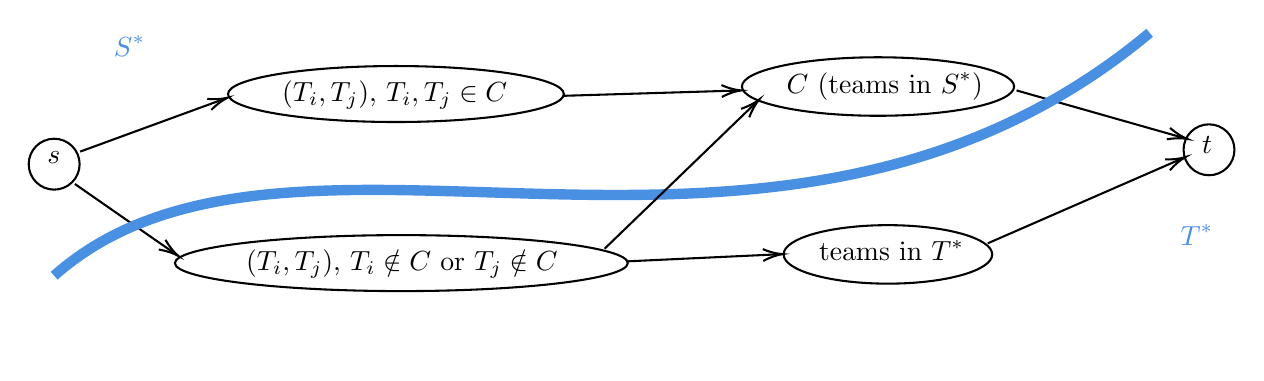
\begin{tikzpicture}[x=0.65pt,y=0.65pt,yscale=-1,xscale=1]
%uncomment if require: \path (0,264); %set diagram left start at 0, and has height of 264

%Straight Lines [id:da7772226935453113] 
\draw    (69,135) -- (149.12,105.69) ;
\draw [shift={(151,105)}, rotate = 159.9] [color={rgb, 255:red, 0; green, 0; blue, 0 }  ][line width=0.75]    (10.93,-3.29) .. controls (6.95,-1.4) and (3.31,-0.3) .. (0,0) .. controls (3.31,0.3) and (6.95,1.4) .. (10.93,3.29)   ;
%Straight Lines [id:da18617385090995575] 
\draw    (66,153) -- (121.86,191.86) ;
\draw [shift={(123.5,193)}, rotate = 214.82] [color={rgb, 255:red, 0; green, 0; blue, 0 }  ][line width=0.75]    (10.93,-3.29) .. controls (6.95,-1.4) and (3.31,-0.3) .. (0,0) .. controls (3.31,0.3) and (6.95,1.4) .. (10.93,3.29)   ;
%Straight Lines [id:da07829298607342994] 
\draw    (573.5,186) -- (681.67,138.8) ;
\draw [shift={(683.5,138)}, rotate = 156.43] [color={rgb, 255:red, 0; green, 0; blue, 0 }  ][line width=0.75]    (10.93,-3.29) .. controls (6.95,-1.4) and (3.31,-0.3) .. (0,0) .. controls (3.31,0.3) and (6.95,1.4) .. (10.93,3.29)   ;
%Straight Lines [id:da9996461500054709] 
\draw    (589.5,101) -- (682.58,127.45) ;
\draw [shift={(684.5,128)}, rotate = 195.87] [color={rgb, 255:red, 0; green, 0; blue, 0 }  ][line width=0.75]    (10.93,-3.29) .. controls (6.95,-1.4) and (3.31,-0.3) .. (0,0) .. controls (3.31,0.3) and (6.95,1.4) .. (10.93,3.29)   ;
%Curve Lines [id:da8046942013314734] 
\draw [color={rgb, 255:red, 74; green, 144; blue, 226 }  ,draw opacity=1 ][line width=3.75]    (54.5,204) .. controls (185.5,88) and (453.5,244) .. (663.5,69) ;
%Straight Lines [id:da7530738110487928] 
\draw    (337.5,104) -- (434.5,101.06) ;
\draw [shift={(436.5,101)}, rotate = 178.26] [color={rgb, 255:red, 0; green, 0; blue, 0 }  ][line width=0.75]    (10.93,-3.29) .. controls (6.95,-1.4) and (3.31,-0.3) .. (0,0) .. controls (3.31,0.3) and (6.95,1.4) .. (10.93,3.29)   ;
%Straight Lines [id:da8123228251562347] 
\draw    (373.5,196) -- (457.5,192.09) ;
\draw [shift={(459.5,192)}, rotate = 177.34] [color={rgb, 255:red, 0; green, 0; blue, 0 }  ][line width=0.75]    (10.93,-3.29) .. controls (6.95,-1.4) and (3.31,-0.3) .. (0,0) .. controls (3.31,0.3) and (6.95,1.4) .. (10.93,3.29)   ;
%Straight Lines [id:da8567126902854119] 
\draw    (360.5,189) -- (445.06,107.39) ;
\draw [shift={(446.5,106)}, rotate = 136.02] [color={rgb, 255:red, 0; green, 0; blue, 0 }  ][line width=0.75]    (10.93,-3.29) .. controls (6.95,-1.4) and (3.31,-0.3) .. (0,0) .. controls (3.31,0.3) and (6.95,1.4) .. (10.93,3.29)   ;

% Text Node
\draw    (244.5, 103) circle [x radius= 93.34, y radius= 15.56]   ;
\draw (179.5,94) node [anchor=north west][inner sep=0.75pt]   [align=left] {$\displaystyle ( T_{i} ,T_{j})$, $\displaystyle T_{i} ,T_{j} \in C$};
% Text Node
\draw    (54.5, 142) circle [x radius= 14.15, y radius= 14.15]   ;
\draw (49,133) node [anchor=north west][inner sep=0.75pt]   [align=left] {$\displaystyle s$};
% Text Node
\draw    (512.5, 98.83) circle [x radius= 75.66, y radius= 16.26]   ;
\draw (460,89.33) node [anchor=north west][inner sep=0.75pt]   [align=left] {$\displaystyle C$ (teams in $\displaystyle S^{*})$};
% Text Node
\draw    (518, 192.16) circle [x radius= 57.98, y radius= 16.26]   ;
\draw (478,182.66) node [anchor=north west][inner sep=0.75pt]   [align=left] {teams in $\displaystyle T^{*}$};
% Text Node
\draw    (696.5, 134) circle [x radius= 14.15, y radius= 14.15]   ;
\draw (691,125) node [anchor=north west][inner sep=0.75pt]   [align=left] {$\displaystyle t$};
% Text Node
\draw (679,174) node [anchor=north west][inner sep=0.75pt]  [color={rgb, 255:red, 74; green, 144; blue, 226 }  ,opacity=1 ] [align=left] {$\displaystyle \textcolor[rgb]{0.29,0.56,0.89}{T}\textcolor[rgb]{0.29,0.56,0.89}{^{*}}$};
% Text Node
\draw (86,69) node [anchor=north west][inner sep=0.75pt]  [color={rgb, 255:red, 74; green, 144; blue, 226 }  ,opacity=1 ] [align=left] {$\displaystyle \textcolor[rgb]{0.29,0.56,0.89}{S}\textcolor[rgb]{0.29,0.56,0.89}{^{*}}$};
% Text Node
\draw    (247.5, 197) circle [x radius= 125.87, y radius= 15.56]   ;
\draw (159.5,188) node [anchor=north west][inner sep=0.75pt]   [align=left] {$\displaystyle ( T_{i} ,T_{j})$, $\displaystyle T_{i} \notin C$ or $\displaystyle T_{j} \notin C$};


\end{tikzpicture}

